% QED3_assembly_outline.tex -- compile with pdflatex twice.
% TikZ conventions adapted from QEO1's overview and RPM1.
\documentclass[11pt]{article}
\usepackage[T1]{fontenc}
\usepackage{lmodern}
\usepackage[paperwidth=22in,paperheight=24in,margin=18mm]{geometry}
\usepackage{amsmath,amssymb}
\usepackage{array,booktabs,tabularx}
\usepackage{xcolor}
\usepackage{tikz}
\usetikzlibrary{arrows.meta,positioning,calc}
\usepackage{enumitem,microtype,fancyhdr}
\definecolor{manuscriptblue}{rgb}{0.1,0.3,0.5}
\definecolor{manuscriptmagenta}{HTML}{60445C}
\definecolor{flowgreen}{HTML}{28764B}
\definecolor{flowgray}{HTML}{62676E}
\usepackage[colorlinks=true,linkcolor=manuscriptmagenta,
 urlcolor=manuscriptblue,pdftitle={QED3 assembly outline},
 pdfsubject={Manuscript structure, main theorems, and dependencies},
 pdfauthor={},bookmarksopen=true]{hyperref}
\urlstyle{same}
\setlength{\parindent}{0pt}
\setlength{\parskip}{5.5pt}
\setlength{\emergencystretch}{2em}
\setlist[itemize]{leftmargin=1.4em,itemsep=2pt,topsep=3pt}
\tikzset{
 proof map/.style={node distance=11mm and 12mm,
   every node/.style={font=\fontsize{10}{12}\selectfont},>=Latex},
 flow base/.style={rectangle,draw=black!65,line width=.55pt,fill=white,
   text=manuscriptmagenta,align=left,text width=82mm,
   minimum height=48mm,inner xsep=3mm,inner ysep=2.5mm,outer sep=1pt},
 flow manuscript/.style={flow base,draw=flowgreen,fill=flowgreen!16},
 flow external/.style={flow base,draw=manuscriptblue,fill=manuscriptblue!9},
 flow target/.style={double=white,double distance=1.1pt},
 flow dependency/.style={draw=black!75,line width=.65pt,
   -{Latex[length=2mm,width=1.3mm]}},
 flow connector/.style={draw=black!75,line width=.65pt},
 flow join/.style={circle,fill=black!75,draw=none,inner sep=0pt,minimum size=3pt},
 flow label/.style={font=\fontsize{9}{11}\selectfont,text=black,
   fill=white,inner sep=2pt,align=center},
 flow annotation/.style={font=\fontsize{9}{11}\selectfont,text=black!75,
   align=left,inner sep=1pt}
}
\newcommand{\FlowHeading}[2]{%
 \hyperlink{block-#1}{\textbf{#1\quad #2}}\par\smallskip}
\newcommand{\Code}[1]{\hyperlink{block-#1}{\textbf{#1}}}
\newcommand{\Block}[2]{\hypertarget{block-#1}{}%
 \subsection*{\textcolor{flowgreen}{#1}\quad #2}}
\newcommand{\ExternalBlock}[2]{\hypertarget{block-#1}{}%
 \subsection*{\textcolor{manuscriptblue}{#1}\quad #2}}
\newcommand{\Inputs}[1]{\textbf{Inputs.} #1\par}
\newcommand{\Theorem}[1]{\textbf{Main theorem.} #1\par}
\newcommand{\Sources}[1]{\par{\small\textcolor{flowgray}{Source material:} #1\par}}
\newcommand{\Repo}{https://github.com/ethanwsussman/Yang--Mills-LLM-experiment}
\newcommand{\Old}[2]{\href{\Repo/#1}{#2}}
\newcommand{\MBsource}{\Old{tree/main/QED3/OLD/Submanuscripts/Maxwell\%20block\%20analysis\%20\%28MB1\%29}{MBM1}}
\newcommand{\FBsource}{\Old{tree/main/QED3/OLD/Submanuscripts/Chamber\%20fermion\%20block\%20analysis\%20\%28FB1\%29}{FBM1}}
\newcommand{\RNsource}{\Old{tree/main/QED3/OLD/Submanuscripts/Relevant\%20extraction\%20and\%20normalized\%20contraction\%20\%28RN1\%29}{RNM1}}
\newcommand{\NLsource}{\Old{tree/main/QED3/OLD/Submanuscripts/Nonlinear\%20renormalization\%20step\%20\%28NL1\%29}{NLM1}}
\newcommand{\CVsource}{\Old{tree/main/QED3/OLD/Submanuscripts/Cover\%20agreement\%20and\%20common\%20tuning\%20\%28CV1\%29}{CVM1}}
\newcommand{\TPsource}{\Old{tree/main/QED3/OLD/Submanuscripts/Terminal\%20measure\%20and\%20pressure\%20\%28TP1\%29}{TPM1}}
\newcommand{\RRsource}{\Old{tree/main/QED3/OLD/Submanuscripts/Reference\%20response\%20\%28RR1\%29}{RRM1}}
\newcommand{\PRsource}{\Old{tree/main/QED3/OLD/Submanuscripts/Positive\%20probes\%20and\%20free\%20response\%20\%28PR1\%29}{PRM1}}
\newcommand{\VTsource}{\Old{tree/main/QED3/OLD/Submanuscripts/Volume\%20transfer\%20\%28VT1\%29}{VTM1}}
\newcommand{\LPsource}{\Old{tree/main/QED3/OLD/Submanuscripts/Infinite-lattice\%20reflection\%20positivity\%20\%28LP1\%29}{LPM1}}
\newcommand{\CEsource}{\Old{tree/main/QED3/OLD/Submanuscripts/Continuum\%20existence\%20\%28CE1\%29}{CEM1}}
\newcommand{\ECsource}{\Old{tree/main/QED3/OLD/Submanuscripts/Continuum\%20components\%20and\%20clustering\%20\%28EC1\%29}{ECM1}}
\newcommand{\RPsource}{\Old{blob/main/RP\%20O\%28d\%29\%20trick\%20\%28RP1\%29/RPM1.tex}{RPM1}}
\newcommand{\QCsource}{\Old{blob/main/QED3/QED3_supplement.tex}{QCM1}}
\newcommand{\QEsource}{\Old{blob/main/QED3/OLD/QEM1.tex}{QEM1}}
\begin{document}
\thispagestyle{empty}
\begin{center}
{\fontsize{16}{19}\selectfont\bfseries QED3 assembly outline}\par
\vspace{3mm}
{\fontsize{11}{14}\selectfont
Lattice positivity, renormalization, and an interacting Osterwalder--Schrader theory}\par
\vspace{2mm}
{\fontsize{10}{12}\selectfont
Spatial volume tends to infinity at fixed lattice spacing; the continuum limit is taken afterwards.}\par
\vspace{7mm}
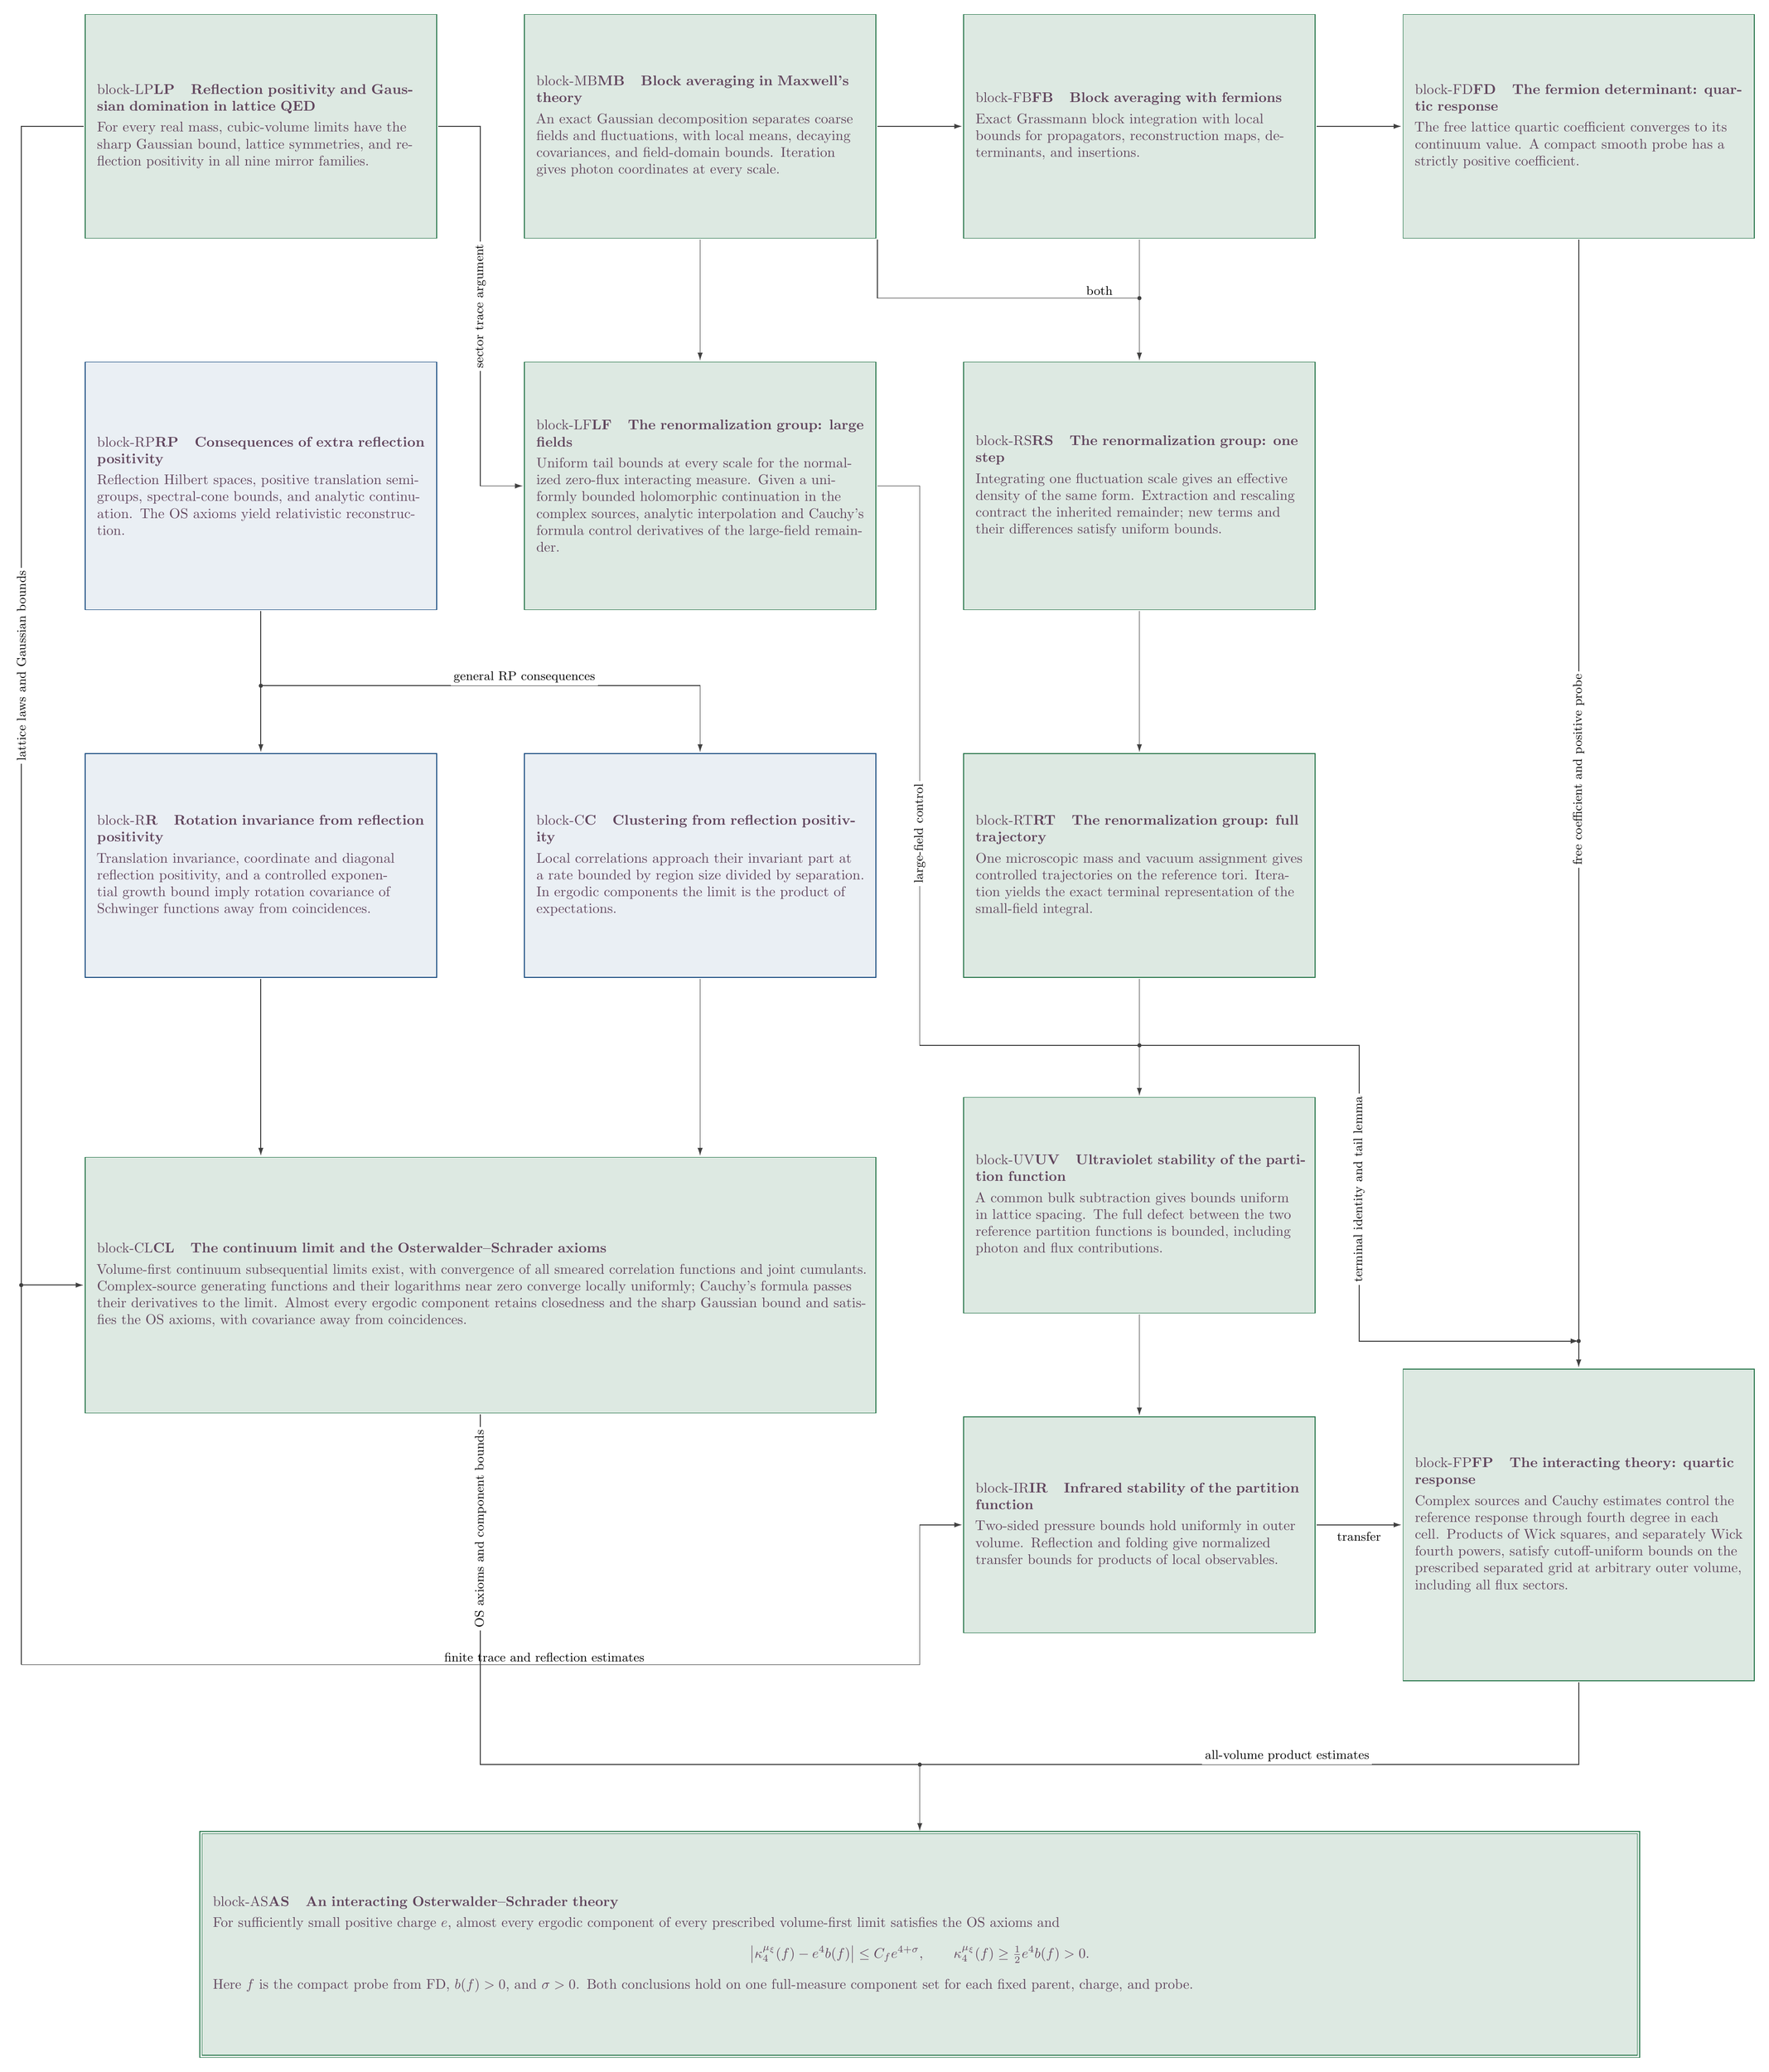
\begin{tikzpicture}[proof map,x=1mm,y=1mm]
 \node[flow manuscript,minimum height=56mm] (LP) at (44,0) {
  \FlowHeading{LP}{Reflection positivity and Gaussian domination in lattice QED}
  For every real mass, cubic-volume limits have the sharp Gaussian bound,
  lattice symmetries, and reflection positivity in all nine mirror families.
 };
 \node[flow manuscript,minimum height=56mm] (MB) at (154,0) {
  \FlowHeading{MB}{Block averaging in Maxwell's theory}
  An exact Gaussian decomposition separates coarse fields and fluctuations,
  with local means, decaying covariances, and field-domain bounds.
  Iteration gives photon coordinates at every scale.
 };
 \node[flow manuscript,minimum height=56mm] (FB) at (264,0) {
  \FlowHeading{FB}{Block averaging with fermions}
  Exact Grassmann block integration with local bounds for propagators,
  reconstruction maps, determinants, and insertions.
 };
 \node[flow manuscript,minimum height=56mm] (FD) at (374,0) {
  \FlowHeading{FD}{The fermion determinant: quartic response}
  The free lattice quartic coefficient converges to its continuum value.
  A compact smooth probe has a strictly positive coefficient.
 };
 \node[flow external,minimum height=62mm] (RP) at (44,-90) {
  \FlowHeading{RP}{Consequences of extra reflection positivity}
  Reflection Hilbert spaces, positive translation semigroups,
  spectral-cone bounds, and analytic continuation.
  The OS axioms yield relativistic reconstruction.
 };
 \node[flow manuscript,minimum height=62mm] (LF) at (154,-90) {
  \FlowHeading{LF}{The renormalization group: large fields}
  Uniform tail bounds at every scale for the normalized zero-flux
  interacting measure. Given a uniformly bounded holomorphic
  continuation in the complex sources, analytic interpolation
  and Cauchy's formula control derivatives of the large-field remainder.
 };
 \node[flow manuscript,minimum height=62mm] (RS) at (264,-90) {
  \FlowHeading{RS}{The renormalization group: one step}
  Integrating one fluctuation scale gives an effective density of the same
  form. Extraction and rescaling contract the inherited remainder;
  new terms and their differences satisfy uniform bounds.
 };
 \node[flow external,minimum height=56mm] (R) at (44,-185) {
  \FlowHeading{R}{Rotation invariance from reflection positivity}
  Translation invariance, coordinate and diagonal reflection positivity,
  and a controlled exponential growth bound imply rotation covariance of Schwinger
  functions away from coincidences.
 };
 \node[flow external,minimum height=56mm] (C) at (154,-185) {
  \FlowHeading{C}{Clustering from reflection positivity}
  Local correlations approach their invariant part at a rate bounded
  by region size divided by separation.
  In ergodic components the limit is the product of expectations.
 };
 \node[flow manuscript,minimum height=56mm] (RT) at (264,-185) {
  \FlowHeading{RT}{The renormalization group: full trajectory}
  One microscopic mass and vacuum assignment gives controlled trajectories
  on the reference tori. Iteration yields the exact terminal representation
  of the small-field integral.
 };
 \node[flow manuscript,text width=192mm,minimum height=64mm] (CL) at (99,-290) {
  \FlowHeading{CL}{The continuum limit and the Osterwalder--Schrader axioms}
  Volume-first continuum subsequential limits exist, with convergence of
  all smeared correlation functions and joint cumulants. Complex-source
  generating functions and their logarithms near zero converge locally
  uniformly; Cauchy's formula passes their derivatives to the limit.
  Almost every ergodic component retains closedness and the sharp Gaussian
  bound and satisfies the OS axioms, with covariance away from coincidences.
 };
 \node[flow manuscript,minimum height=54mm] (UV) at (264,-270) {
  \FlowHeading{UV}{Ultraviolet stability of the partition function}
  A common bulk subtraction gives bounds uniform in lattice spacing.
  The full defect between the two reference partition functions is
  bounded, including photon and flux contributions.
 };
 \node[flow manuscript,minimum height=54mm] (IR) at (264,-350) {
  \FlowHeading{IR}{Infrared stability of the partition function}
  Two-sided pressure bounds hold uniformly in outer volume.
  Reflection and folding give normalized transfer bounds
  for products of local observables.
 };
 \node[flow manuscript,minimum height=78mm] (FP) at (374,-350) {
  \FlowHeading{FP}{The interacting theory: quartic response}
  Complex sources and Cauchy estimates control the reference response
  through fourth degree in each cell. Products of Wick squares,
  and separately Wick fourth
  powers, satisfy cutoff-uniform bounds on the prescribed separated grid
  at arbitrary outer volume, including all flux sectors.
 };
 \node[flow manuscript,flow target,text width=354mm,minimum height=56mm] (AS) at (209,-455) {
  \FlowHeading{AS}{An interacting Osterwalder--Schrader theory}
  For sufficiently small positive charge \(e\), almost every ergodic component
  of every prescribed volume-first limit satisfies the OS axioms and
  \[
   \bigl|\kappa_4^{\mu_\xi}(f)-e^4b(f)\bigr|\le C_f e^{4+\sigma},
   \qquad
   \kappa_4^{\mu_\xi}(f)\ge \tfrac12e^4b(f)>0.
  \]
  Here \(f\) is the compact probe from FD, \(b(f)>0\), and \(\sigma>0\).
  Both conclusions hold on one full-measure component set
  for each fixed parent, charge, and probe.
 };

 % Primitive estimates and one-step integration.
 \draw[flow dependency] (MB.east) -- (FB.west);
 \draw[flow dependency] (FB.east) -- (FD.west);
 \coordinate (rsjoin) at (264,-43);
 \draw[flow dependency] (MB.south) -- (LF.north);
 \draw[flow connector] (MB.south east) -- (MB.south east |- rsjoin) -- (rsjoin);
 \draw[flow connector] (FB.south) -- (rsjoin);
 \node[flow join] at (rsjoin) {};
 \draw[flow dependency] (rsjoin) -- (RS.north);
 \node[flow label,anchor=south] at (254,-43) {both};

 % Shared lattice trace foundation; sector restriction stays in LF's proof.
 \draw[flow dependency] (LP.east) -- (99,0) -- (99,-90) -- (LF.west);
 \node[flow label,rotate=90] at (99,-45) {sector trace argument};
 \draw[flow connector] (LP.west) -- (-16,0) -- (-16,-385);
 \draw[flow dependency] (-16,-290) -- (CL.west);
 \node[flow join] at (-16,-290) {};
 \draw[flow dependency] (-16,-385) -- (209,-385) -- (209,-350) -- (IR.west);
 \node[flow label,rotate=90] at (-16,-135) {lattice laws and Gaussian bounds};
 \node[flow label,anchor=south] at (115,-385) {finite trace and reflection estimates};

 % External general branch.
 \coordinate (rpjoin) at (44,-140);
 \draw[flow connector] (RP.south) -- (rpjoin);
 \draw[flow dependency] (rpjoin) -- (R.north);
 \draw[flow dependency] (rpjoin) -- (154,-140) -- (C.north);
 \node[flow join] at (rpjoin) {};
 \node[flow label,anchor=south] at (110,-140) {general RP consequences};
 \draw[flow dependency] (R.south) -- (R.south |- CL.north);
 \draw[flow dependency] (C.south) -- (C.south |- CL.north);

 % Trajectory and independent large-field bounds feed both UV and FP.
 \draw[flow dependency] (RS.south) -- (RT.north);
 \coordinate (uvjoin) at (264,-230);
 \draw[flow connector] (RT.south) -- (uvjoin);
 \draw[flow connector] (LF.east) -- (209,-90) -- (209,-230) -- (uvjoin);
 \node[flow label,rotate=90] at (209,-177) {large-field control};
 \node[flow join] at (uvjoin) {};
 \draw[flow dependency] (uvjoin) -- (UV.north);
 \draw[flow dependency] (UV.south) -- (IR.north);
 \coordinate (fpjoin) at (374,-304);
 \draw[flow dependency] (uvjoin) -- (319,-230) -- (319,-304) -- (fpjoin);
 \node[flow label,rotate=90] at (319,-266) {terminal identity and tail lemma};
 \draw[flow connector] (FD.south) -- (fpjoin);
 \node[flow label,rotate=90] at (374,-161) {free coefficient and positive probe};
 \node[flow join] at (fpjoin) {};
 \draw[flow dependency] (fpjoin) -- (FP.north);
 \draw[flow dependency] (IR.east) -- (FP.west);
 \node[flow label,anchor=north] at (319,-351) {transfer};

 % Final application to the same parent and its components.
 \coordinate (asjoin) at (209,-410);
 \draw[flow connector] (CL.south) -- (99,-410) -- (asjoin);
 \draw[flow connector] (FP.south) -- (374,-410) -- (asjoin);
 \node[flow join] at (asjoin) {};
 \draw[flow dependency] (asjoin) -- (AS.north);
 \node[flow label,rotate=90] at (99,-351) {OS axioms and component bounds};
 \node[flow label,anchor=south] at (301,-410) {all-volume product estimates};
\end{tikzpicture}
\par\vspace{4mm}
{\fontsize{10}{12}\selectfont
\tikz[baseline=-.5ex]\node[draw=flowgreen,fill=flowgreen!16,
 minimum width=5mm,minimum height=3mm,inner sep=0pt]{};
\enspace Construction manuscript or final assembly
\qquad
\tikz[baseline=-.5ex]\node[draw=manuscriptblue,fill=manuscriptblue!9,
 minimum width=5mm,minimum height=3mm,inner sep=0pt]{};
\enspace External general theorem\par\smallskip
Arrows show principal dependencies. Joined inputs are required together;
crossings without a dot do not join.}
\end{center}

% Ordinary reading pages after the QEO1-sized overview sheet.
\clearpage
\pdfpagewidth=210mm
\pdfpageheight=297mm
\setlength{\paperwidth}{210mm}
\setlength{\paperheight}{297mm}
\newgeometry{layoutwidth=210mm,layoutheight=297mm,left=20mm,right=20mm,top=20mm,bottom=20mm,headheight=14pt,headsep=6mm,footskip=10mm}
\pagestyle{fancy}
\fancyhf{}
\fancyhead[L]{\small QED3 assembly outline}
\fancyhead[R]{\small Main theorems and dependencies}
\fancyfoot[C]{\small\thepage}
\renewcommand{\headrulewidth}{.3pt}
\setcounter{page}{2}
\section*{The program and its endpoint}
\begin{center}
\small\renewcommand{\arraystretch}{1.18}
\begin{tabularx}{\textwidth}{@{}l l X@{}}
\toprule
& Code & Manuscript or result\\
\midrule
1 & \Code{MB} & Block averaging in Maxwell's theory\\
2 & \Code{FB} & Block averaging with fermions\\
3 & \Code{RS} & The renormalization group: one step\\
4 & \Code{RT} & The renormalization group: full trajectory\\
5 & \Code{LF} & The renormalization group: large fields\\
6 & \Code{UV} & Ultraviolet stability of the partition function\\
7 & \Code{IR} & Infrared stability of the partition function\\
8 & \Code{FD} & The fermion determinant: quartic response\\
9 & \Code{FP} & The interacting theory: quartic response\\
\midrule
& \Code{LP} & Reflection positivity and Gaussian domination in lattice QED\\
& \Code{CL} & The continuum limit and the Osterwalder--Schrader axioms\\
\midrule
External & \Code{RP} & Consequences of extra reflection positivity\\
External & \Code{R} & Rotation invariance from reflection positivity\\
External & \Code{C} & Clustering from reflection positivity\\
\midrule
Assembly & \Code{AS} & An interacting Osterwalder--Schrader theory\\
\bottomrule
\end{tabularx}
\end{center}
\textbf{Order of limits.}
At each fixed lattice spacing \(a>0\), first let the spatial size tend to
infinity and choose an infinite-volume limit. Then take a subsequential
limit as \(a\downarrow0\).

\textbf{Final result.}
Fix an admitted positive reference mass and chamber parameters.
For sufficiently small positive physical charge \(e\), the common
microscopic parameters selected by \Code{RT} give volume-first continuum
subsequential limits of the all-flux curvature laws, with convergence of
all smeared correlation functions and joint cumulants.
For every such parent, almost every
translation-ergodic component \(\mu_\xi\) is a closed real tempered field,
retains the sharp Gaussian bound, and has Schwinger functions satisfying
the OS axioms, including clustering.

For the fixed compact smooth probe \(f\) supplied by \Code{FD}, the same
component set satisfies
\[
 \left|\kappa_4^{\mu_\xi}(f)-e^4b(f)\right|
 \le C_f e^{4+\sigma},
 \qquad \kappa_4^{\mu_\xi}(f)\ge \tfrac12e^4b(f)>0.
\]
Here \(\kappa_4\) is the connected fourth moment of the smeared curvature,
\(b(f)>0\), and \(\sigma>0\). The components are non-Gaussian.
Both conclusions hold on one full-measure component set for each fixed
parent, charge, and probe.
\Sources{\QEsource, field-strength theorem; \VTsource, component cumulant theorem.}


\clearpage
\section*{Block averaging and renormalization}

\Block{MB}{Block averaging in Maxwell's theory}
\Inputs{The Maxwell quadratic form, gauge fixing, and block geometry.}
\Theorem{An exact normalized Gaussian decomposition separates the photon
field into a coarse background and independent fluctuations. The
constrained means, covariances, and local inverses satisfy uniform
locality, decay, regularity, and field-domain bounds. Iteration gives
photon fluctuation coordinates at every scale.}
\Sources{\MBsource; photon coordinates in \TPsource.}

\Block{FB}{Block averaging with fermions}
\Inputs{\Code{MB} and the chamber fermion operator in an admissible
complex background connection.}
\Theorem{An exact Grassmann block-integration identity gives uniform
local bounds for propagators, fluctuation covariances, and reconstruction
maps. Determinant contributions and marked insertions satisfy the bounds
used in scale iteration and terminal integration.}
\Sources{\FBsource; reconstruction in \RNsource; terminal estimates in \TPsource.}

\Block{RS}{The renormalization group: one step}
\Inputs{\Code{MB}, \Code{FB}, an admitted running mass, and a small local
interaction on the specified field domain.}
\Theorem{Integrating one restricted fluctuation scale produces an exact
effective density of the same form, with updated mass, vacuum energy,
background scalar terms, and interaction. Extraction and rescaling
contract the normalized inherited remainder. Newly generated terms and
their differences satisfy the iteration bounds.
The local transformation agrees on admissible covers.}
\Sources{\RNsource, \NLsource, and the local comparison estimates in \CVsource.}

\Block{RT}{The renormalization group: full trajectory}
\Inputs{\Code{RS}.}
\Theorem{For each cutoff, one microscopic mass and vacuum-energy
assignment gives a controlled trajectory through the stopping scales
on every torus in the reference family. The assignment is independent
of the external probe and harmonic twist. Iteration expresses the
small-field integral exactly as a terminal measure, retaining sources,
bounded measurable observables, and normalization factors.}
\Sources{\CVsource; terminal measure identity in \TPsource.}

\clearpage
\section*{Large fields and partition stability}

\Block{LF}{The renormalization group: large fields}
\Inputs{Photon coordinates from \Code{MB} and the finite-volume trace
construction from \Code{LP}.}
\Theorem{The normalized zero-flux interacting measure assigns small
probability to the excluded fluctuation and terminal-curvature
configurations on the reference volumes, uniformly in the ultraviolet
cutoff and the initial real mass and vacuum parameters.
Given a holomorphic continuation of the excluded contribution with
a uniform complex-source bound, its smallness for real sources extends
by analytic interpolation to a smaller complex neighborhood.
Cauchy's formula then controls its source derivatives.}
\Sources{\TPsource, zero-flux domination and terminal tails;
analytic interpolation and Cauchy estimates in \RRsource.}

\Block{UV}{Ultraviolet stability of the partition function}
\Inputs{\Code{RT}, \Code{LF}, and terminal fermion estimates from \Code{FB}.}
\Theorem{After a common cutoff-dependent bulk subtraction, the reference
partition functions satisfy bounds uniform in lattice spacing.
At fixed physical charge, the full defect between the two reference
partition functions is bounded uniformly in the ultraviolet cutoff,
including the photon determinant and magnetic-flux contributions.}
\Sources{Partition estimates in \TPsource; full partition defect in \VTsource, \S3.}

\Block{IR}{Infrared stability of the partition function}
\Inputs{The reference partition bound from \Code{UV} and the trace,
reflection, and folding identities from \Code{LP}.}
\Theorem{One common bulk subtraction gives upper and lower bounds on
the logarithm of the partition function per physical volume, uniformly
over arbitrarily large admissible tori. Folding gives a normalized
transfer inequality for products of local observables, with normalization
cost controlled by the reference partition defect.}
\Sources{\VTsource, \S2 and the general transfer proposition.}

\Block{FD}{The fermion determinant: quartic response}
\Inputs{The free chamber symbol, heavy-mode gap, Schur complement,
and inverse estimates from \Code{FB}.}
\Theorem{The fourth logarithmic derivative of the free lattice fermion
determinant converges to its continuum value. The second and fourth
derivatives of the normalized determinant ratio satisfy uniform bounds.
There is a real compact smooth curvature probe \(f\) with strictly
positive continuum quartic coefficient \(b(f)\).}
\Sources{\PRsource, positive-probe and free-response theorems.}

\clearpage
\section*{The four-point function and continuum limits}

\Block{FP}{The interacting theory: quartic response}
\Inputs{\Code{RT}, \Code{FB}, \Code{LF}, \Code{FD}, and \Code{IR}.}
\Theorem{The source-shift identity expresses Wick correlations as
derivatives of a normalized complex-source generating function.
On the reference torus, analytic estimates and Cauchy's formula bound
the difference between its mixed derivatives and their free values,
through degree four in each cell. The resulting bounds for finite
products of Wick squares,
and separately Wick fourth powers, transfer to distinct cells of the
prescribed separated grid on arbitrarily large admissible tori.
The bounds are uniform in the cutoffs and include all magnetic-flux
sectors. The source identity and terminal logarithm estimates supply
the complex bound used in \Code{LF} to differentiate the large-field
remainder.}
\Sources{Complex-source identities and response estimates in \RRsource;
all-volume Wick-product bounds in \VTsource.}

\Block{LP}{Reflection positivity and Gaussian domination in lattice QED}
\Inputs{The all-flux chamber lattice model at fixed lattice parameters.}
\Theorem{For every real mass, the cubic finite-volume curvature laws
are tight. Every subsequential limit along integer cubic side lengths
tending to infinity obeys the sharp Gaussian bound, lattice translations
and cubic symmetries, and reflection positivity in the three coordinate
and six diagonal mirror families. The reflection form is positive for
all square-integrable observables supported strictly on either side.}
\Sources{\LPsource, main theorem.}

\Block{CL}{The continuum limit and the Osterwalder--Schrader axioms}
\Inputs{\Code{LP}, \Code{RP}, \Code{R}, and \Code{C}.}
\Theorem{Volume-first continuum subsequential limits exist, and
\emph{all smeared correlation functions and joint cumulants converge}
along the chosen limiting sequences. For each finite family of Schwartz tests,
the complex-source generating functions converge locally uniformly,
as do their logarithms on a common zero-free neighborhood of zero.
Gaussian domination supplies the
uniform complex bounds; Cauchy's formula passes source derivatives
to the limit.

Each prescribed parent is a closed real tempered two-form law with
the sharp Gaussian bound. Almost every translation-ergodic
component retains the same Gaussian constant and the reflection forms.
Its Schwinger functions satisfy OS regularity, Euclidean covariance away
from coincidences, reflection positivity, permutation symmetry, and
clustering.}
\Sources{Complex-source convergence and continuum existence in \CEsource;
component inheritance in \ECsource;
supported tensor tests in \QEsource.}

\clearpage
\section*{External theorems and assembly}

\ExternalBlock{RP}{Consequences of extra reflection positivity}
\Inputs{Translation invariance, coordinate and diagonal reflection
forms, and the field-insertion bound
\(\mathbb E e^{F(f)}\le\exp\{C(\|f\|_1+\|f\|_2^2)\}\).}
\Theorem{Coordinate reflection positivity gives reflection Hilbert
spaces and positive translation semigroups. Diagonal reflection
positivity gives spectral-cone bounds and identifies the zero-energy
projections with the invariant part. The exponential bound gives
analytic translations, continuation of correlation kernels, and
extension to polynomial and supported tensor tests.
The OS axioms yield relativistic reconstruction.}
\Sources{Reflection and analytic arguments in \RPsource;
tensor-test and reconstruction arguments in \QEsource\ and \QCsource.}

\ExternalBlock{R}{Rotation invariance from reflection positivity}
\Inputs{\Code{RP}, translation invariance, coordinate and diagonal
reflection positivity, the exponential bound in \Code{RP}, and an orthogonal
tensor representation with planar weights \(\lvert w\rvert\le2\).}
\Theorem{The Schwinger functions are covariant under continuous
rotations away from coincident configurations.}
\Sources{\RPsource, Theorem A.}

\ExternalBlock{C}{Clustering from reflection positivity}
\Inputs{Translation invariance, invariance and reflection positivity
in the nine coordinate and diagonal orientations, and the spectral
results of \Code{RP}.}
\Theorem{Local correlations approach their translation-invariant
conditional part. For observables supported in a cube of radius \(r\)
and separated by \(\lvert a\rvert_\infty\ge4r\), the error is bounded by
a universal constant times \(r/\lvert a\rvert_\infty\) and the product
of their \(L^2\) norms. Qualitative mixing holds for all \(L^2\)
observables. For an ergodic law the limit is the product of expectations.}
\Sources{The clustering appendix in \QCsource;
invariant projections in \ECsource.}

\Block{AS}{An interacting Osterwalder--Schrader theory}
\Inputs{\Code{CL} and \Code{FP}, with the parameters from \Code{RT}
and the probe from \Code{FD}.}
\Theorem{For sufficiently small positive charge, almost every ergodic
component of every prescribed volume-first parent satisfies the OS
axioms and the positive fourth-cumulant estimate on page~2.
Both conclusions hold on one full-measure component set for each
fixed parent, charge, and probe.}
\Sources{Component cumulants in \VTsource; assembly in \QEsource.}

\clearpage
\section*{Where the existing material goes}
\par\small\renewcommand{\arraystretch}{1.2}
\begin{tabularx}{\textwidth}{@{}p{31mm} X@{}}
\toprule
Existing material & Destination and role\\
\midrule
\MBsource & \Code{MB}: exact photon decomposition and local estimates.\\
\FBsource & \Code{FB}: fermion integration, inverses, determinants, and
background estimates.\\
\RNsource & \Code{RS}: extraction and contraction; general reconstruction
bounds move with \Code{FB}.\\
\NLsource & \Code{RS}: exact nonlinear fluctuation integration and its
remainder estimates.\\
\CVsource & \Code{RT}: common tuning and controlled trajectories;
local cover compatibility accompanies \Code{RS}.\\
\TPsource & \Code{MB}: iterated photon coordinates.
\Code{FB}: general terminal fermion estimates.
\Code{RT}: exact terminal identity.
\Code{LF}: zero-flux domination and excluded-field tails.
\Code{UV}: reference partition comparison.\\
\RRsource & \Code{FP}: complex-source identities, Cauchy estimates, and
the interacting remainder. \Code{LF}: analytic interpolation of tail bounds.\\
\PRsource & \Code{FD}: free second/fourth response and the positive probe.\\
\VTsource & \Code{UV}: full photon/flux partition defect.
\Code{IR}: pressure bounds and general observable transfer.
\Code{FP}: all-flux Wick products and conditional component transfer.
\Code{AS}: application to the selected continuum components.\\
\LPsource & \Code{LP}: lattice construction and reflection positivity.\\
\CEsource & \Code{CL}: compactness, prescribed-parent recovery, and
convergence of correlations and cumulants by complex sources and Cauchy's formula.\\
\ECsource & \Code{CL}: component reflection forms and sharp Gaussian bound.
\Code{RP}, \Code{C}: general cone, invariant-projection, and clustering results.\\
\RPsource & \Code{R}: rotations. \Code{RP}: spectral and analytic results.\\
\QCsource & \Code{C}: quantitative clustering. \Code{RP}: analytic continuation and reconstruction.\\
\QEsource & \Code{CL}: supported tensor tests. \Code{AS}: parameter admission and assembly.\\
\bottomrule
\end{tabularx}
\par\normalsize
\end{document}
